% Options for packages loaded elsewhere
\PassOptionsToPackage{unicode}{hyperref}
\PassOptionsToPackage{hyphens}{url}
\PassOptionsToPackage{dvipsnames,svgnames,x11names}{xcolor}
%
\documentclass[
  letterpaper,
  DIV=11,
  numbers=noendperiod]{scrreprt}

\usepackage{amsmath,amssymb}
\usepackage{iftex}
\ifPDFTeX
  \usepackage[T1]{fontenc}
  \usepackage[utf8]{inputenc}
  \usepackage{textcomp} % provide euro and other symbols
\else % if luatex or xetex
  \usepackage{unicode-math}
  \defaultfontfeatures{Scale=MatchLowercase}
  \defaultfontfeatures[\rmfamily]{Ligatures=TeX,Scale=1}
\fi
\usepackage{lmodern}
\ifPDFTeX\else  
    % xetex/luatex font selection
\fi
% Use upquote if available, for straight quotes in verbatim environments
\IfFileExists{upquote.sty}{\usepackage{upquote}}{}
\IfFileExists{microtype.sty}{% use microtype if available
  \usepackage[]{microtype}
  \UseMicrotypeSet[protrusion]{basicmath} % disable protrusion for tt fonts
}{}
\makeatletter
\@ifundefined{KOMAClassName}{% if non-KOMA class
  \IfFileExists{parskip.sty}{%
    \usepackage{parskip}
  }{% else
    \setlength{\parindent}{0pt}
    \setlength{\parskip}{6pt plus 2pt minus 1pt}}
}{% if KOMA class
  \KOMAoptions{parskip=half}}
\makeatother
\usepackage{xcolor}
\setlength{\emergencystretch}{3em} % prevent overfull lines
\setcounter{secnumdepth}{5}
% Make \paragraph and \subparagraph free-standing
\ifx\paragraph\undefined\else
  \let\oldparagraph\paragraph
  \renewcommand{\paragraph}[1]{\oldparagraph{#1}\mbox{}}
\fi
\ifx\subparagraph\undefined\else
  \let\oldsubparagraph\subparagraph
  \renewcommand{\subparagraph}[1]{\oldsubparagraph{#1}\mbox{}}
\fi

\usepackage{color}
\usepackage{fancyvrb}
\newcommand{\VerbBar}{|}
\newcommand{\VERB}{\Verb[commandchars=\\\{\}]}
\DefineVerbatimEnvironment{Highlighting}{Verbatim}{commandchars=\\\{\}}
% Add ',fontsize=\small' for more characters per line
\usepackage{framed}
\definecolor{shadecolor}{RGB}{241,243,245}
\newenvironment{Shaded}{\begin{snugshade}}{\end{snugshade}}
\newcommand{\AlertTok}[1]{\textcolor[rgb]{0.68,0.00,0.00}{#1}}
\newcommand{\AnnotationTok}[1]{\textcolor[rgb]{0.37,0.37,0.37}{#1}}
\newcommand{\AttributeTok}[1]{\textcolor[rgb]{0.40,0.45,0.13}{#1}}
\newcommand{\BaseNTok}[1]{\textcolor[rgb]{0.68,0.00,0.00}{#1}}
\newcommand{\BuiltInTok}[1]{\textcolor[rgb]{0.00,0.23,0.31}{#1}}
\newcommand{\CharTok}[1]{\textcolor[rgb]{0.13,0.47,0.30}{#1}}
\newcommand{\CommentTok}[1]{\textcolor[rgb]{0.37,0.37,0.37}{#1}}
\newcommand{\CommentVarTok}[1]{\textcolor[rgb]{0.37,0.37,0.37}{\textit{#1}}}
\newcommand{\ConstantTok}[1]{\textcolor[rgb]{0.56,0.35,0.01}{#1}}
\newcommand{\ControlFlowTok}[1]{\textcolor[rgb]{0.00,0.23,0.31}{#1}}
\newcommand{\DataTypeTok}[1]{\textcolor[rgb]{0.68,0.00,0.00}{#1}}
\newcommand{\DecValTok}[1]{\textcolor[rgb]{0.68,0.00,0.00}{#1}}
\newcommand{\DocumentationTok}[1]{\textcolor[rgb]{0.37,0.37,0.37}{\textit{#1}}}
\newcommand{\ErrorTok}[1]{\textcolor[rgb]{0.68,0.00,0.00}{#1}}
\newcommand{\ExtensionTok}[1]{\textcolor[rgb]{0.00,0.23,0.31}{#1}}
\newcommand{\FloatTok}[1]{\textcolor[rgb]{0.68,0.00,0.00}{#1}}
\newcommand{\FunctionTok}[1]{\textcolor[rgb]{0.28,0.35,0.67}{#1}}
\newcommand{\ImportTok}[1]{\textcolor[rgb]{0.00,0.46,0.62}{#1}}
\newcommand{\InformationTok}[1]{\textcolor[rgb]{0.37,0.37,0.37}{#1}}
\newcommand{\KeywordTok}[1]{\textcolor[rgb]{0.00,0.23,0.31}{#1}}
\newcommand{\NormalTok}[1]{\textcolor[rgb]{0.00,0.23,0.31}{#1}}
\newcommand{\OperatorTok}[1]{\textcolor[rgb]{0.37,0.37,0.37}{#1}}
\newcommand{\OtherTok}[1]{\textcolor[rgb]{0.00,0.23,0.31}{#1}}
\newcommand{\PreprocessorTok}[1]{\textcolor[rgb]{0.68,0.00,0.00}{#1}}
\newcommand{\RegionMarkerTok}[1]{\textcolor[rgb]{0.00,0.23,0.31}{#1}}
\newcommand{\SpecialCharTok}[1]{\textcolor[rgb]{0.37,0.37,0.37}{#1}}
\newcommand{\SpecialStringTok}[1]{\textcolor[rgb]{0.13,0.47,0.30}{#1}}
\newcommand{\StringTok}[1]{\textcolor[rgb]{0.13,0.47,0.30}{#1}}
\newcommand{\VariableTok}[1]{\textcolor[rgb]{0.07,0.07,0.07}{#1}}
\newcommand{\VerbatimStringTok}[1]{\textcolor[rgb]{0.13,0.47,0.30}{#1}}
\newcommand{\WarningTok}[1]{\textcolor[rgb]{0.37,0.37,0.37}{\textit{#1}}}

\providecommand{\tightlist}{%
  \setlength{\itemsep}{0pt}\setlength{\parskip}{0pt}}\usepackage{longtable,booktabs,array}
\usepackage{calc} % for calculating minipage widths
% Correct order of tables after \paragraph or \subparagraph
\usepackage{etoolbox}
\makeatletter
\patchcmd\longtable{\par}{\if@noskipsec\mbox{}\fi\par}{}{}
\makeatother
% Allow footnotes in longtable head/foot
\IfFileExists{footnotehyper.sty}{\usepackage{footnotehyper}}{\usepackage{footnote}}
\makesavenoteenv{longtable}
\usepackage{graphicx}
\makeatletter
\def\maxwidth{\ifdim\Gin@nat@width>\linewidth\linewidth\else\Gin@nat@width\fi}
\def\maxheight{\ifdim\Gin@nat@height>\textheight\textheight\else\Gin@nat@height\fi}
\makeatother
% Scale images if necessary, so that they will not overflow the page
% margins by default, and it is still possible to overwrite the defaults
% using explicit options in \includegraphics[width, height, ...]{}
\setkeys{Gin}{width=\maxwidth,height=\maxheight,keepaspectratio}
% Set default figure placement to htbp
\makeatletter
\def\fps@figure{htbp}
\makeatother

\KOMAoption{captions}{tableheading}
\makeatletter
\makeatother
\makeatletter
\@ifpackageloaded{bookmark}{}{\usepackage{bookmark}}
\makeatother
\makeatletter
\@ifpackageloaded{caption}{}{\usepackage{caption}}
\AtBeginDocument{%
\ifdefined\contentsname
  \renewcommand*\contentsname{Table of contents}
\else
  \newcommand\contentsname{Table of contents}
\fi
\ifdefined\listfigurename
  \renewcommand*\listfigurename{List of Figures}
\else
  \newcommand\listfigurename{List of Figures}
\fi
\ifdefined\listtablename
  \renewcommand*\listtablename{List of Tables}
\else
  \newcommand\listtablename{List of Tables}
\fi
\ifdefined\figurename
  \renewcommand*\figurename{Figure}
\else
  \newcommand\figurename{Figure}
\fi
\ifdefined\tablename
  \renewcommand*\tablename{Table}
\else
  \newcommand\tablename{Table}
\fi
}
\@ifpackageloaded{float}{}{\usepackage{float}}
\floatstyle{ruled}
\@ifundefined{c@chapter}{\newfloat{codelisting}{h}{lop}}{\newfloat{codelisting}{h}{lop}[chapter]}
\floatname{codelisting}{Listing}
\newcommand*\listoflistings{\listof{codelisting}{List of Listings}}
\makeatother
\makeatletter
\@ifpackageloaded{caption}{}{\usepackage{caption}}
\@ifpackageloaded{subcaption}{}{\usepackage{subcaption}}
\makeatother
\makeatletter
\@ifpackageloaded{tcolorbox}{}{\usepackage[skins,breakable]{tcolorbox}}
\makeatother
\makeatletter
\@ifundefined{shadecolor}{\definecolor{shadecolor}{rgb}{.97, .97, .97}}
\makeatother
\makeatletter
\makeatother
\makeatletter
\makeatother
\ifLuaTeX
  \usepackage{selnolig}  % disable illegal ligatures
\fi
\IfFileExists{bookmark.sty}{\usepackage{bookmark}}{\usepackage{hyperref}}
\IfFileExists{xurl.sty}{\usepackage{xurl}}{} % add URL line breaks if available
\urlstyle{same} % disable monospaced font for URLs
\hypersetup{
  pdftitle={R para el análisis estadístico de datos},
  pdfauthor={Ana Escoto},
  colorlinks=true,
  linkcolor={blue},
  filecolor={Maroon},
  citecolor={Blue},
  urlcolor={Blue},
  pdfcreator={LaTeX via pandoc}}

\title{R para el análisis estadístico de datos}
\author{Ana Escoto}
\date{2024-10-06}

\begin{document}
\maketitle
\ifdefined\Shaded\renewenvironment{Shaded}{\begin{tcolorbox}[interior hidden, sharp corners, frame hidden, borderline west={3pt}{0pt}{shadecolor}, enhanced, breakable, boxrule=0pt]}{\end{tcolorbox}}\fi

\renewcommand*\contentsname{Table of contents}
{
\hypersetup{linkcolor=}
\setcounter{tocdepth}{2}
\tableofcontents
}
\bookmarksetup{startatroot}

\hypertarget{sobre-el-curso}{%
\chapter*{Sobre el curso}\label{sobre-el-curso}}
\addcontentsline{toc}{chapter}{Sobre el curso}

\markboth{Sobre el curso}{Sobre el curso}

\hypertarget{introducciuxf3n-a-r-y-rstudio-4-horas}{%
\section*{Introducción a R y Rstudio (4
horas)}\label{introducciuxf3n-a-r-y-rstudio-4-horas}}
\addcontentsline{toc}{section}{Introducción a R y Rstudio (4 horas)}

\markright{Introducción a R y Rstudio (4 horas)}

\emph{Objetivo: que el estudiantado sea familiarice con la interfase de
trabajo y la programación por objetos, del mismo modo que sean capaces
de realizar tareas básicas tales como crear un script, un proyecto,
objetos, ambientes e instalar paqueterías}.

\hypertarget{importaciuxf3n-de-informaciuxf3n-y-primera-revisiuxf3n-de-fuentes-demogruxe1ficas-4-horas}{%
\section*{Importación de información y primera revisión de fuentes
demográficas (4
horas)}\label{importaciuxf3n-de-informaciuxf3n-y-primera-revisiuxf3n-de-fuentes-demogruxe1ficas-4-horas}}
\addcontentsline{toc}{section}{Importación de información y primera
revisión de fuentes demográficas (4 horas)}

\markright{Importación de información y primera revisión de fuentes
demográficas (4 horas)}

\begin{enumerate}
\def\labelenumi{\alph{enumi}.}
\item
  Importación de información a R en diferentes formatos
\item
  Revisión de encuestas y ejemplos de importación de datos en formatos
  diferentes
\item
  Revisión preliminar y limpieza de información
\end{enumerate}

\emph{Objetivo: que el estudiantado sea capaz de importar información
desde diferentes formatos (.txt, .csv, .xlsx, .dta, .dbf) a R, así como
de exportar sus resultados en estos formatos. Del mismo modo que sean
capaces de revisar de manera preliminar los objetos de tipo
\texttt{data.frame}: funciones \texttt{dplyr::glimpse()},
\texttt{skimr::skim()}, manejo de etiquetas y hacer subconjuntos de
información}

\hypertarget{revisiuxf3n-de-elementos-estaduxedsticos-buxe1sicos-desde-tidyverse-8-horas}{%
\section*{Revisión de elementos estadísticos básicos desde ``tidyverse''
(8
horas)}\label{revisiuxf3n-de-elementos-estaduxedsticos-buxe1sicos-desde-tidyverse-8-horas}}
\addcontentsline{toc}{section}{Revisión de elementos estadísticos
básicos desde ``tidyverse'' (8 horas)}

\markright{Revisión de elementos estadísticos básicos desde
``tidyverse'' (8 horas)}

\begin{enumerate}
\def\labelenumi{\alph{enumi}.}
\item
  Tabulados con \texttt{janitor::tabyl()} y uso de factores de expansión
  con \texttt{pollster::topline()}, \texttt{pollstter::crosstab}.
  Lectura e interpretación de tablas de doble entrada
\item
  Estadística descriptiva básica (medidas de tendencia central,
  dispersión y de posición) con el paquete \texttt{\{dplyr\}}
\item
  Gráficos univariados y bivariados usando \texttt{\{ggplot2\}} y
  extensiones de \texttt{\{ggplot2\}}
\item
  Fusionado de información
\end{enumerate}

\emph{Objetivo: que el estudiantado sea capaz de realizar análisis
estadísticos básicos utilizando encuenstas mexicanas}

\hypertarget{estimaciones-por-intervalo-y-diseuxf1o-complejo-muestral-4-horas}{%
\section*{Estimaciones por intervalo y diseño complejo muestral (4
horas)}\label{estimaciones-por-intervalo-y-diseuxf1o-complejo-muestral-4-horas}}
\addcontentsline{toc}{section}{Estimaciones por intervalo y diseño
complejo muestral (4 horas)}

\markright{Estimaciones por intervalo y diseño complejo muestral (4
horas)}

\begin{enumerate}
\def\labelenumi{\alph{enumi}.}
\item
  Estimaciones para medias
\item
  Estimaciones para proporciones
\item
  Estimaciones para totales
\item
  Estimaciones lineales de coeficientes
\end{enumerate}

\emph{Objetivo: que el estudiantado sea capaz de realizar intervalos de
confianza, calculo de errores estándar con diseño muestral complejo y
sepa evaluar la confiabilidad de sus estimaciones}

\bookmarksetup{startatroot}

\hypertarget{facilitadora}{%
\chapter*{Facilitadora}\label{facilitadora}}
\addcontentsline{toc}{chapter}{Facilitadora}

\markboth{Facilitadora}{Facilitadora}

\hypertarget{ana-ruth-escoto-castillo}{%
\section*{Ana Ruth Escoto Castillo}\label{ana-ruth-escoto-castillo}}
\addcontentsline{toc}{section}{Ana Ruth Escoto Castillo}

\markright{Ana Ruth Escoto Castillo}

Profesora de tiempo completo en la Facultad de Ciencias Políticas y
Sociales, UNAM. Doctora en Estudios de Población por El Colegio de
México, cuenta con el nivel I en el Sistema Nacional de Investigadores.
Coorganizadora del capítulo de la CDMX de la iniciativa global Rladies.
Le interesa el bienestar de la población, en el presente, analizando los
procesos de desigualdad y exclusión en los mercados laborales
latinoamericanos; y, en el futuro, a través del estudio de la
sustentabilidad. Su experiencia en el ámbito académico se ha concentrado
en el estudio de este bienestar, específicamente en el análisis
sociodemográfico de las condiciones laborales y la vinculación del
comercio exterior con el mercado de trabajo, en la relación del cambio
climático y la distribución de ingresos, el consumo energético de los
hogares y sus implicaciones ambientales. Posee experiencia en
recolección de información estadística, diseño y control de procesos de
recolección y su procesamiento. Ha aplicado diversos métodos y
herramientas multivariadas, homologación de información y comparabilidad
de fuentes en sus investigaciones, así como usa de diversos softwares
estadísticos, y ha impartido clases de estadítica aplicada a nivel de
licenciatura y posgrado.

\bookmarksetup{startatroot}

\hypertarget{instalaciuxf3n-de-r-y-rstudio}{%
\chapter*{Instalación de R y
Rstudio}\label{instalaciuxf3n-de-r-y-rstudio}}
\addcontentsline{toc}{chapter}{Instalación de R y Rstudio}

\markboth{Instalación de R y Rstudio}{Instalación de R y Rstudio}

\hypertarget{introducciuxf3n-a-r}{%
\section*{Introducción a R}\label{introducciuxf3n-a-r}}
\addcontentsline{toc}{section}{Introducción a R}

\markright{Introducción a R}

\url{https://youtu.be/YkN5urybh2A}

\hypertarget{instalaciuxf3n-en-os}{%
\section*{Instalación en OS}\label{instalaciuxf3n-en-os}}
\addcontentsline{toc}{section}{Instalación en OS}

\markright{Instalación en OS}

\begin{enumerate}
\def\labelenumi{\arabic{enumi}.}
\tightlist
\item
  Necesito que instalen la versión más nueva de R: Download R-4.4.0 of
  MAC. \emph{The R-project for statistical computing}.
  \url{https://cran.r-project.org/bin/macosx/}
\end{enumerate}

Elije la versión de acuerdo a tu procesador, intel o ARM.

\begin{enumerate}
\def\labelenumi{\arabic{enumi}.}
\setcounter{enumi}{1}
\tightlist
\item
  Instalar también las herramientas Quartz, xcode y fortran
\end{enumerate}

\begin{itemize}
\item
  \url{https://www.xquartz.org/}
\item
  \url{https://developer.apple.com/xcode/resources/}
\item
  \url{https://mac.r-project.org/tools/gfortran-12.2-universal.pkg}
\end{itemize}

\begin{enumerate}
\def\labelenumi{\arabic{enumi}.}
\setcounter{enumi}{2}
\tightlist
\item
  Después de eso instalar el Rstudio, que hoy se encuentra alojado en el
  sitio posit, que vaya acorde con MAC
\end{enumerate}

\url{https://posit.co/download/rstudio-desktop/}

Algunas indicaciones en video, pero son algo viejitas y pueden cambiar
las versiones de R.

\url{https://youtu.be/icWV8jzYOtA}

Algunas indicaciones en video, pero son algo viejitas y pueden cambiar
las versiones de R.

\hypertarget{instalaciuxf3n-en-pc}{%
\section*{Instalación en PC}\label{instalaciuxf3n-en-pc}}
\addcontentsline{toc}{section}{Instalación en PC}

\markright{Instalación en PC}

\begin{enumerate}
\def\labelenumi{\arabic{enumi}.}
\item
  Necesito que instalen la versión más nueva de R: Download R-4.4.0 for
  Windows. \emph{The R-project for statistical computing}.
  \url{https://cran.r-project.org/bin/windows/base/}
\item
  Instalar también la herramienta RTools
  \url{https://cran.r-project.org/bin/windows/Rtools/rtools44/rtools.html}
\item
  Después de eso instalar el Rstudio, que hoy se encuentra alojado en el
  sitio posit, que vaya acorde con Windows
  \url{https://posit.co/download/rstudio-desktop/}
\end{enumerate}

Algunas indicaciones en video, pero son algo viejitas y pueden cambiar
las versiones de R.

\url{https://youtu.be/TNSQikMfgJI}

\hypertarget{ojo}{%
\section*{Ojo}\label{ojo}}
\addcontentsline{toc}{section}{Ojo}

\markright{Ojo}

Desde octubre de 2022, RStudio se volvió \textbf{``Posit''}

\bookmarksetup{startatroot}

\hypertarget{primer-acercamiento-al-uso-del-programa}{%
\chapter{Primer acercamiento al uso del
programa}\label{primer-acercamiento-al-uso-del-programa}}

\hypertarget{introducciuxf3n}{%
\section{Introducción}\label{introducciuxf3n}}

En RStudio podemos tener varias ventanas que nos permiten tener más
control de nuestro ``ambiente'', el historial, los ``scripts'' o códigos
que escribimos y por supuesto, tenemos nuestra consola, que también
tiene el símbolo ``\textgreater{}'' con R. Podemos pedir operaciones
básicas

\begin{Shaded}
\begin{Highlighting}[]
\DecValTok{2}\SpecialCharTok{+}\DecValTok{5}
\end{Highlighting}
\end{Shaded}

\begin{verbatim}
[1] 7
\end{verbatim}

\begin{Shaded}
\begin{Highlighting}[]
\DecValTok{5}\SpecialCharTok{*}\DecValTok{3}
\end{Highlighting}
\end{Shaded}

\begin{verbatim}
[1] 15
\end{verbatim}

\begin{Shaded}
\begin{Highlighting}[]
\CommentTok{\#Para escribir comentarios y que no los lea como operaciones ponemos el símbolo de gato}
\CommentTok{\# Lo podemos hacer para un comentario en una línea o la par de una instrucción}

\DecValTok{1}\SpecialCharTok{:}\DecValTok{5}               \CommentTok{\# Secuencia 1{-}5}
\end{Highlighting}
\end{Shaded}

\begin{verbatim}
[1] 1 2 3 4 5
\end{verbatim}

\begin{Shaded}
\begin{Highlighting}[]
\FunctionTok{seq}\NormalTok{(}\DecValTok{1}\NormalTok{, }\DecValTok{10}\NormalTok{, }\FloatTok{0.5}\NormalTok{)   }\CommentTok{\# Secuencia con incrementos diferentes a 1}
\end{Highlighting}
\end{Shaded}

\begin{verbatim}
 [1]  1.0  1.5  2.0  2.5  3.0  3.5  4.0  4.5  5.0  5.5  6.0  6.5  7.0  7.5  8.0
[16]  8.5  9.0  9.5 10.0
\end{verbatim}

\begin{Shaded}
\begin{Highlighting}[]
\FunctionTok{c}\NormalTok{(}\StringTok{\textquotesingle{}a\textquotesingle{}}\NormalTok{,}\StringTok{\textquotesingle{}b\textquotesingle{}}\NormalTok{,}\StringTok{\textquotesingle{}c\textquotesingle{}}\NormalTok{)  }\CommentTok{\# Vector con caracteres}
\end{Highlighting}
\end{Shaded}

\begin{verbatim}
[1] "a" "b" "c"
\end{verbatim}

\begin{Shaded}
\begin{Highlighting}[]
\DecValTok{1}\SpecialCharTok{:}\DecValTok{7}             \CommentTok{\# Entero}
\end{Highlighting}
\end{Shaded}

\begin{verbatim}
[1] 1 2 3 4 5 6 7
\end{verbatim}

\begin{Shaded}
\begin{Highlighting}[]
\DecValTok{40} \SpecialCharTok{\textless{}} \DecValTok{80}         \CommentTok{\# Valor logico}
\end{Highlighting}
\end{Shaded}

\begin{verbatim}
[1] TRUE
\end{verbatim}

\begin{Shaded}
\begin{Highlighting}[]
\DecValTok{2} \SpecialCharTok{+} \DecValTok{2} \SpecialCharTok{==} \DecValTok{5}      \CommentTok{\# Valor logico}
\end{Highlighting}
\end{Shaded}

\begin{verbatim}
[1] FALSE
\end{verbatim}

\begin{Shaded}
\begin{Highlighting}[]
\NormalTok{T }\SpecialCharTok{==} \ConstantTok{TRUE}       \CommentTok{\# T expresion corta de verdadero}
\end{Highlighting}
\end{Shaded}

\begin{verbatim}
[1] TRUE
\end{verbatim}

R es un lenguaje de programación por objetos. Por lo cual vamos a tener
objetos a los que se les asigna su contenido. Si usamos una flechita
``\textless-'' o ``-\textgreater{}'' le estamos asignando algo al objeto
que apunta la felcha.

\begin{Shaded}
\begin{Highlighting}[]
\NormalTok{x }\OtherTok{\textless{}{-}} \DecValTok{24}         \CommentTok{\# Asignacion de valor 24 a la variable x para su uso posterior (OBJETO)}
\NormalTok{x}\SpecialCharTok{/}\DecValTok{2}             \CommentTok{\# Uso posterior de variable u objeto x}
\end{Highlighting}
\end{Shaded}

\begin{verbatim}
[1] 12
\end{verbatim}

\begin{Shaded}
\begin{Highlighting}[]
\NormalTok{x               }\CommentTok{\# Imprime en pantalla el valor de la variable u objeto}
\end{Highlighting}
\end{Shaded}

\begin{verbatim}
[1] 24
\end{verbatim}

\begin{Shaded}
\begin{Highlighting}[]
\NormalTok{x }\OtherTok{\textless{}{-}} \ConstantTok{TRUE}       \CommentTok{\# Asigna el valor logico TRUE a la variable x OJO: x toma el ultimo valor que se le asigna}
\NormalTok{x}
\end{Highlighting}
\end{Shaded}

\begin{verbatim}
[1] TRUE
\end{verbatim}

\hypertarget{vectores}{%
\section{Vectores}\label{vectores}}

Los vectores son uno de los objetos más usados en R.

\begin{Shaded}
\begin{Highlighting}[]
\NormalTok{y }\OtherTok{\textless{}{-}} \FunctionTok{c}\NormalTok{(}\DecValTok{2}\NormalTok{, }\DecValTok{4}\NormalTok{, }\DecValTok{6}\NormalTok{)     }\CommentTok{\# Vector numerico}
\NormalTok{y }\OtherTok{\textless{}{-}} \FunctionTok{c}\NormalTok{(}\StringTok{\textquotesingle{}Primaria\textquotesingle{}}\NormalTok{, }\StringTok{\textquotesingle{}Secundaria\textquotesingle{}}\NormalTok{) }\CommentTok{\# Vector caracteres}
\end{Highlighting}
\end{Shaded}

Dado que poseen elementos, podemos también observar y hacer operaciones
con sus elementos, usando ``{[} {]}'' para acceder a ellos

\begin{Shaded}
\begin{Highlighting}[]
\NormalTok{y[}\DecValTok{2}\NormalTok{]              }\CommentTok{\# Acceder al segundo valor del vector y}
\end{Highlighting}
\end{Shaded}

\begin{verbatim}
[1] "Secundaria"
\end{verbatim}

\begin{Shaded}
\begin{Highlighting}[]
\NormalTok{y[}\DecValTok{3}\NormalTok{] }\OtherTok{\textless{}{-}} \StringTok{\textquotesingle{}Preparatoria y más\textquotesingle{}} \CommentTok{\# Asigna valor a la tercera componente del vector}
\NormalTok{sex }\OtherTok{\textless{}{-}}\DecValTok{1}\SpecialCharTok{:}\DecValTok{2}         \CommentTok{\# Asigna a la variable sex los valores 1 y 2}
\FunctionTok{names}\NormalTok{(sex) }\OtherTok{\textless{}{-}} \FunctionTok{c}\NormalTok{(}\StringTok{"Femenino"}\NormalTok{, }\StringTok{"Masculino"}\NormalTok{) }\CommentTok{\# Asigna nombres al vector de elementos sexo}
\NormalTok{sex[}\DecValTok{2}\NormalTok{]            }\CommentTok{\# Segundo elemento del vector sex}
\end{Highlighting}
\end{Shaded}

\begin{verbatim}
Masculino 
        2 
\end{verbatim}

\hypertarget{matrices}{%
\section{Matrices}\label{matrices}}

Las matrices son muy importantes, porque nos permiten hacer operaciones
y casi todas nuestras bases de datos tendran un aspecto de matriz.

\begin{Shaded}
\begin{Highlighting}[]
\NormalTok{m }\OtherTok{\textless{}{-}} \FunctionTok{matrix}\NormalTok{ (}\AttributeTok{nrow=}\DecValTok{2}\NormalTok{, }\AttributeTok{ncol=}\DecValTok{3}\NormalTok{, }\DecValTok{1}\SpecialCharTok{:}\DecValTok{6}\NormalTok{, }\AttributeTok{byrow =} \ConstantTok{TRUE}\NormalTok{) }\CommentTok{\# Matrices Ejemplo 1}
\NormalTok{m}
\end{Highlighting}
\end{Shaded}

\begin{verbatim}
     [,1] [,2] [,3]
[1,]    1    2    3
[2,]    4    5    6
\end{verbatim}

\begin{Shaded}
\begin{Highlighting}[]
\NormalTok{m }\OtherTok{\textless{}{-}} \FunctionTok{matrix}\NormalTok{ (}\AttributeTok{nrow=}\DecValTok{2}\NormalTok{, }\AttributeTok{ncol=}\DecValTok{3}\NormalTok{, }\DecValTok{1}\SpecialCharTok{:}\DecValTok{6}\NormalTok{, }\AttributeTok{byrow =} \ConstantTok{FALSE}\NormalTok{) }\CommentTok{\# Matrices Ejemplo 1}
\NormalTok{m}
\end{Highlighting}
\end{Shaded}

\begin{verbatim}
     [,1] [,2] [,3]
[1,]    1    3    5
[2,]    2    4    6
\end{verbatim}

\begin{Shaded}
\begin{Highlighting}[]
\FunctionTok{dim}\NormalTok{(m)}
\end{Highlighting}
\end{Shaded}

\begin{verbatim}
[1] 2 3
\end{verbatim}

\begin{Shaded}
\begin{Highlighting}[]
\FunctionTok{attributes}\NormalTok{(m)}
\end{Highlighting}
\end{Shaded}

\begin{verbatim}
$dim
[1] 2 3
\end{verbatim}

¿Qué hace ``byrow''?

\begin{Shaded}
\begin{Highlighting}[]
\NormalTok{n }\OtherTok{\textless{}{-}} \DecValTok{1}\SpecialCharTok{:}\DecValTok{6}     \CommentTok{\# Matrices Ejemplo 2}
\FunctionTok{dim}\NormalTok{(n) }\OtherTok{\textless{}{-}} \FunctionTok{c}\NormalTok{(}\DecValTok{2}\NormalTok{,}\DecValTok{3}\NormalTok{)}
\NormalTok{n}
\end{Highlighting}
\end{Shaded}

\begin{verbatim}
     [,1] [,2] [,3]
[1,]    1    3    5
[2,]    2    4    6
\end{verbatim}

\begin{Shaded}
\begin{Highlighting}[]
\NormalTok{xx }\OtherTok{\textless{}{-}}\DecValTok{10}\SpecialCharTok{:}\DecValTok{12}   \CommentTok{\# Matrices Ejemplo 3}
\NormalTok{yy}\OtherTok{\textless{}{-}}\DecValTok{14}\SpecialCharTok{:}\DecValTok{16}
\FunctionTok{cbind}\NormalTok{(xx,yy) }\CommentTok{\# Une vectores por Columnas}
\end{Highlighting}
\end{Shaded}

\begin{verbatim}
     xx yy
[1,] 10 14
[2,] 11 15
[3,] 12 16
\end{verbatim}

\begin{Shaded}
\begin{Highlighting}[]
\FunctionTok{rbind}\NormalTok{(xx,yy) }\CommentTok{\# Une vectores por Renglones}
\end{Highlighting}
\end{Shaded}

\begin{verbatim}
   [,1] [,2] [,3]
xx   10   11   12
yy   14   15   16
\end{verbatim}

\begin{Shaded}
\begin{Highlighting}[]
\NormalTok{mi\_matrix}\OtherTok{\textless{}{-}}\FunctionTok{cbind}\NormalTok{(xx,yy) }\CommentTok{\# este resultado lo puedo asignar a un objeto}
\end{Highlighting}
\end{Shaded}

\hypertarget{data.frames-o-conjuntos-de-datos}{%
\section{data.frames o conjuntos de
datos}\label{data.frames-o-conjuntos-de-datos}}

\begin{Shaded}
\begin{Highlighting}[]
\NormalTok{mi\_dataframe}\OtherTok{\textless{}{-}}\FunctionTok{as.data.frame}\NormalTok{(m)}
\end{Highlighting}
\end{Shaded}

El formato matricial sigue sirviendo:

\begin{Shaded}
\begin{Highlighting}[]
\NormalTok{mi\_dataframe[}\DecValTok{2}\NormalTok{,]}
\end{Highlighting}
\end{Shaded}

\begin{verbatim}
  V1 V2 V3
2  2  4  6
\end{verbatim}

\begin{Shaded}
\begin{Highlighting}[]
\NormalTok{mi\_dataframe[,}\DecValTok{2}\NormalTok{]}
\end{Highlighting}
\end{Shaded}

\begin{verbatim}
[1] 3 4
\end{verbatim}

Pero también podemos utilizar el símbolo de peso para cada variable:

\begin{Shaded}
\begin{Highlighting}[]
\NormalTok{mi\_dataframe}\SpecialCharTok{$}\NormalTok{V2}
\end{Highlighting}
\end{Shaded}

\begin{verbatim}
[1] 3 4
\end{verbatim}

Puedo agregar variables columnas:

\begin{Shaded}
\begin{Highlighting}[]
\FunctionTok{cbind}\NormalTok{(mi\_dataframe, }\FunctionTok{c}\NormalTok{(}\StringTok{"a"}\NormalTok{, }\StringTok{"b"}\NormalTok{), }\FunctionTok{c}\NormalTok{(T, F))}
\end{Highlighting}
\end{Shaded}

\begin{verbatim}
  V1 V2 V3 c("a", "b") c(T, F)
1  1  3  5           a    TRUE
2  2  4  6           b   FALSE
\end{verbatim}

Qué pasa con las matrices

\begin{Shaded}
\begin{Highlighting}[]
\FunctionTok{cbind}\NormalTok{(m, }\FunctionTok{c}\NormalTok{(}\StringTok{"a"}\NormalTok{, }\StringTok{"b"}\NormalTok{),  }\FunctionTok{c}\NormalTok{(T, F))}
\end{Highlighting}
\end{Shaded}

\begin{verbatim}
     [,1] [,2] [,3] [,4] [,5]   
[1,] "1"  "3"  "5"  "a"  "TRUE" 
[2,] "2"  "4"  "6"  "b"  "FALSE"
\end{verbatim}

Checa cómo cambian los elementos. En una matriz todos los elementos
deben ser del mismo tipo.

Podemos crear ``a mano'' dataframes:

\begin{Shaded}
\begin{Highlighting}[]
\NormalTok{data}\OtherTok{\textless{}{-}}\FunctionTok{data.frame}\NormalTok{(}
  \StringTok{"entero"} \OtherTok{=} \DecValTok{1}\SpecialCharTok{:}\DecValTok{4}\NormalTok{, }
  \StringTok{"factor"} \OtherTok{=} \FunctionTok{as.factor}\NormalTok{(}\FunctionTok{c}\NormalTok{(}\StringTok{"a"}\NormalTok{, }\StringTok{"b"}\NormalTok{, }\StringTok{"c"}\NormalTok{, }\StringTok{"d"}\NormalTok{)), }
  \StringTok{"numero"} \OtherTok{=} \FunctionTok{c}\NormalTok{(}\DecValTok{1}\SpecialCharTok{/}\DecValTok{1}\NormalTok{, }\DecValTok{1}\SpecialCharTok{/}\DecValTok{2}\NormalTok{, }\DecValTok{1}\SpecialCharTok{/}\DecValTok{3}\NormalTok{, }\DecValTok{1}\SpecialCharTok{/}\DecValTok{4}\NormalTok{),}
  \StringTok{"cadena"} \OtherTok{=} \FunctionTok{as.character}\NormalTok{(}\FunctionTok{c}\NormalTok{(}\StringTok{"a"}\NormalTok{, }\StringTok{"b"}\NormalTok{, }\StringTok{"c"}\NormalTok{, }\StringTok{"d"}\NormalTok{))}
\NormalTok{)}
\end{Highlighting}
\end{Shaded}

Los data.frames tienen una estructura

\begin{Shaded}
\begin{Highlighting}[]
\FunctionTok{str}\NormalTok{(data)}
\end{Highlighting}
\end{Shaded}

\begin{verbatim}
'data.frame':   4 obs. of  4 variables:
 $ entero: int  1 2 3 4
 $ factor: Factor w/ 4 levels "a","b","c","d": 1 2 3 4
 $ numero: num  1 0.5 0.333 0.25
 $ cadena: chr  "a" "b" "c" "d"
\end{verbatim}

\hypertarget{valores-y-perdidos}{%
\section{Valores y perdidos}\label{valores-y-perdidos}}

Además de caracteres, numéricos y lógicos hay también valores perdidos.
Y de varios tipos

\begin{Shaded}
\begin{Highlighting}[]
\NormalTok{vector}\OtherTok{\textless{}{-}}\FunctionTok{c}\NormalTok{(}\DecValTok{1}\SpecialCharTok{:}\DecValTok{5}\NormalTok{, }\CommentTok{\# numérico}
\NormalTok{          T, }\CommentTok{\# lógico}
          \ConstantTok{NA}\NormalTok{, }\CommentTok{\# perdido}
          \StringTok{"a"}\NormalTok{, }\CommentTok{\# caracter}
          \DecValTok{5}\SpecialCharTok{/}\DecValTok{0}\NormalTok{, }\CommentTok{\# no es un número}
          \FunctionTok{sqrt}\NormalTok{(}\SpecialCharTok{{-}}\DecValTok{1}\NormalTok{))}
\end{Highlighting}
\end{Shaded}

\begin{verbatim}
Warning in sqrt(-1): Se han producido NaNs
\end{verbatim}

Si lo imprimimos vamos a ir viendo cómo se convierten ciertos valores a
otros al quererlos incluir en un mismo conjunto:

\begin{Shaded}
\begin{Highlighting}[]
\NormalTok{vector}
\end{Highlighting}
\end{Shaded}

\begin{verbatim}
 [1] "1"    "2"    "3"    "4"    "5"    "TRUE" NA     "a"    "Inf"  "NaN" 
\end{verbatim}

Quitaremos el caracter

\begin{Shaded}
\begin{Highlighting}[]
\NormalTok{vector}\OtherTok{\textless{}{-}}\FunctionTok{c}\NormalTok{(}\DecValTok{1}\SpecialCharTok{:}\DecValTok{5}\NormalTok{, }\CommentTok{\# numérico}
\NormalTok{          T, }\CommentTok{\# lógico}
          \ConstantTok{NA}\NormalTok{, }\CommentTok{\# perdido}
          \DecValTok{5}\SpecialCharTok{/}\DecValTok{0}\NormalTok{, }\CommentTok{\# Infinito}
          \FunctionTok{sqrt}\NormalTok{(}\SpecialCharTok{{-}}\DecValTok{1}\NormalTok{))}
\end{Highlighting}
\end{Shaded}

\begin{verbatim}
Warning in sqrt(-1): Se han producido NaNs
\end{verbatim}

\begin{Shaded}
\begin{Highlighting}[]
\NormalTok{vector}
\end{Highlighting}
\end{Shaded}

\begin{verbatim}
[1]   1   2   3   4   5   1  NA Inf NaN
\end{verbatim}

¿Qué le pasó al valor lógico?

Hay unos operadores que nos señalan si los valores son perdidos o
infinitos o ``Not a number''

\begin{Shaded}
\begin{Highlighting}[]
\FunctionTok{is.na}\NormalTok{(vector)}
\end{Highlighting}
\end{Shaded}

\begin{verbatim}
[1] FALSE FALSE FALSE FALSE FALSE FALSE  TRUE FALSE  TRUE
\end{verbatim}

\begin{Shaded}
\begin{Highlighting}[]
\FunctionTok{is.nan}\NormalTok{(vector)}
\end{Highlighting}
\end{Shaded}

\begin{verbatim}
[1] FALSE FALSE FALSE FALSE FALSE FALSE FALSE FALSE  TRUE
\end{verbatim}

\begin{Shaded}
\begin{Highlighting}[]
\FunctionTok{is.infinite}\NormalTok{(vector)}
\end{Highlighting}
\end{Shaded}

\begin{verbatim}
[1] FALSE FALSE FALSE FALSE FALSE FALSE FALSE  TRUE FALSE
\end{verbatim}

\hypertarget{funciones}{%
\section{Funciones}\label{funciones}}

Algunas funciones básicas son las siguientes. Vamos a ir viendo más
funciones, pero para entender cómo funcionan, haremos unos ejemplos y
cómo pedir ayuda sobre ellas.

\begin{Shaded}
\begin{Highlighting}[]
\FunctionTok{sum}\NormalTok{(}\DecValTok{10}\NormalTok{, }\DecValTok{20}\NormalTok{, }\DecValTok{30}\NormalTok{)    }\CommentTok{\# Función suma}
\end{Highlighting}
\end{Shaded}

\begin{verbatim}
[1] 60
\end{verbatim}

\begin{Shaded}
\begin{Highlighting}[]
\FunctionTok{rep}\NormalTok{(}\StringTok{\textquotesingle{}R\textquotesingle{}}\NormalTok{, }\AttributeTok{times =} \DecValTok{3}\NormalTok{) }\CommentTok{\# Repite la letra R el numero de veces que se indica}
\end{Highlighting}
\end{Shaded}

\begin{verbatim}
[1] "R" "R" "R"
\end{verbatim}

\begin{Shaded}
\begin{Highlighting}[]
\FunctionTok{sqrt}\NormalTok{(}\DecValTok{9}\NormalTok{)           }\CommentTok{\# Raiz cuadrada de 9}
\end{Highlighting}
\end{Shaded}

\begin{verbatim}
[1] 3
\end{verbatim}

\hypertarget{listas}{%
\section{Listas}\label{listas}}

Las listas son conjuntos de objetos y pueden ser de varios tipos

\begin{Shaded}
\begin{Highlighting}[]
\NormalTok{milista}\OtherTok{\textless{}{-}} \FunctionTok{list}\NormalTok{(data, m, xx, }\StringTok{"a"}\NormalTok{)}
\end{Highlighting}
\end{Shaded}

\begin{Shaded}
\begin{Highlighting}[]
\NormalTok{milista}
\end{Highlighting}
\end{Shaded}

\begin{verbatim}
[[1]]
  entero factor    numero cadena
1      1      a 1.0000000      a
2      2      b 0.5000000      b
3      3      c 0.3333333      c
4      4      d 0.2500000      d

[[2]]
     [,1] [,2] [,3]
[1,]    1    3    5
[2,]    2    4    6

[[3]]
[1] 10 11 12

[[4]]
[1] "a"
\end{verbatim}

Ojo con los corchetes

\begin{Shaded}
\begin{Highlighting}[]
\NormalTok{milista[[}\DecValTok{1}\NormalTok{]]}
\end{Highlighting}
\end{Shaded}

\begin{verbatim}
  entero factor    numero cadena
1      1      a 1.0000000      a
2      2      b 0.5000000      b
3      3      c 0.3333333      c
4      4      d 0.2500000      d
\end{verbatim}

Si queremos ponerle nombres a los elementos

\begin{Shaded}
\begin{Highlighting}[]
\NormalTok{milista}\OtherTok{\textless{}{-}} \FunctionTok{list}\NormalTok{(}\AttributeTok{datos =}\NormalTok{ data, }
               \AttributeTok{matriz =}\NormalTok{ m, }
               \AttributeTok{vector =}\NormalTok{ xx,}
               \AttributeTok{valor =} \StringTok{"a"}\NormalTok{)}

\NormalTok{milista}
\end{Highlighting}
\end{Shaded}

\begin{verbatim}
$datos
  entero factor    numero cadena
1      1      a 1.0000000      a
2      2      b 0.5000000      b
3      3      c 0.3333333      c
4      4      d 0.2500000      d

$matriz
     [,1] [,2] [,3]
[1,]    1    3    5
[2,]    2    4    6

$vector
[1] 10 11 12

$valor
[1] "a"
\end{verbatim}

\hypertarget{ayuda}{%
\section{Ayuda}\label{ayuda}}

Pedir ayuda es indispensable para aprender a escribir nuestros códigos.
A prueba y error, es el mejor sistema para aprender. Podemos usar la
función help, example y ?

\begin{Shaded}
\begin{Highlighting}[]
\FunctionTok{help}\NormalTok{(sum)         }\CommentTok{\# Ayuda sobre función sum}
\FunctionTok{example}\NormalTok{(sum)      }\CommentTok{\# Ejemplo de función sum}
\end{Highlighting}
\end{Shaded}

\begin{verbatim}

sum> ## Pass a vector to sum, and it will add the elements together.
sum> sum(1:5)
[1] 15

sum> ## Pass several numbers to sum, and it also adds the elements.
sum> sum(1, 2, 3, 4, 5)
[1] 15

sum> ## In fact, you can pass vectors into several arguments, and everything gets added.
sum> sum(1:2, 3:5)
[1] 15

sum> ## If there are missing values, the sum is unknown, i.e., also missing, ....
sum> sum(1:5, NA)
[1] NA

sum> ## ... unless  we exclude missing values explicitly:
sum> sum(1:5, NA, na.rm = TRUE)
[1] 15
\end{verbatim}

\hypertarget{mi-ambiente}{%
\section{Mi ambiente}\label{mi-ambiente}}

Todos los objetos que hemos declarado hasta ahora son parte de nuestro
``ambiente'' (environment). Para saber qué está en nuestro ambiente
usamos el comando

\begin{Shaded}
\begin{Highlighting}[]
\FunctionTok{ls}\NormalTok{()}
\end{Highlighting}
\end{Shaded}

\begin{verbatim}
 [1] "data"            "has_annotations" "m"               "mi_dataframe"   
 [5] "mi_matrix"       "milista"         "n"               "pandoc_dir"     
 [9] "quarto_bin_path" "sex"             "vector"          "x"              
[13] "xx"              "y"               "yy"             
\end{verbatim}

\begin{Shaded}
\begin{Highlighting}[]
\FunctionTok{gc}\NormalTok{()           }\CommentTok{\# Garbage collection, reporta memoria en uso}
\end{Highlighting}
\end{Shaded}

\begin{verbatim}
          used (Mb) gc trigger (Mb) limit (Mb) max used (Mb)
Ncells  624953 33.4    1330177 71.1         NA  1330177 71.1
Vcells 1173516  9.0    8388608 64.0      16384  2128434 16.3
\end{verbatim}

Para borrar todos nuestros objetos, usamos el siguiente comando, que
equivale a usar la escobita de la venta de environment

\begin{Shaded}
\begin{Highlighting}[]
\FunctionTok{rm}\NormalTok{(}\AttributeTok{list=}\FunctionTok{ls}\NormalTok{())  }\CommentTok{\# Borrar objetos actuales}
\end{Highlighting}
\end{Shaded}

\hypertarget{directorio-de-trabajo}{%
\section{Directorio de trabajo}\label{directorio-de-trabajo}}

Es muy útil saber dónde estamos trabajando y donde queremos trabajar.
Por eso podemos utilizar los siguientes comandos para saberlo

Ojo, checa, si estás desdes una PC, cómo cambian las ``\,'' por''/'' o
por ``\textbackslash{}''

\begin{Shaded}
\begin{Highlighting}[]
\FunctionTok{getwd}\NormalTok{()           }\CommentTok{\# Directorio actual}
\end{Highlighting}
\end{Shaded}

\begin{verbatim}
[1] "/Users/anaescoto/Dropbox/2024/Curso_R_inter/r_analisis_datos/r_analisis_datos"
\end{verbatim}

\begin{Shaded}
\begin{Highlighting}[]
\CommentTok{\#setwd("")\# Cambio de directorio}

\FunctionTok{list.files}\NormalTok{()      }\CommentTok{\# Lista de archivos en ese directorio}
\end{Highlighting}
\end{Shaded}

\begin{verbatim}
 [1] "P1.html"                "P1.qmd"                 "P1.rmarkdown"          
 [4] "P1_files"               "README.md"              "_quarto.yml"           
 [7] "datos"                  "docs"                   "index.html"            
[10] "index.qmd"              "index.tex"              "instala.html"          
[13] "instala.qmd"            "intro1.png"             "r_analisis_datos.Rproj"
[16] "site_libs"             
\end{verbatim}

Checar que esto también se puede hacer desde el menú:

\begin{figure}

{\centering 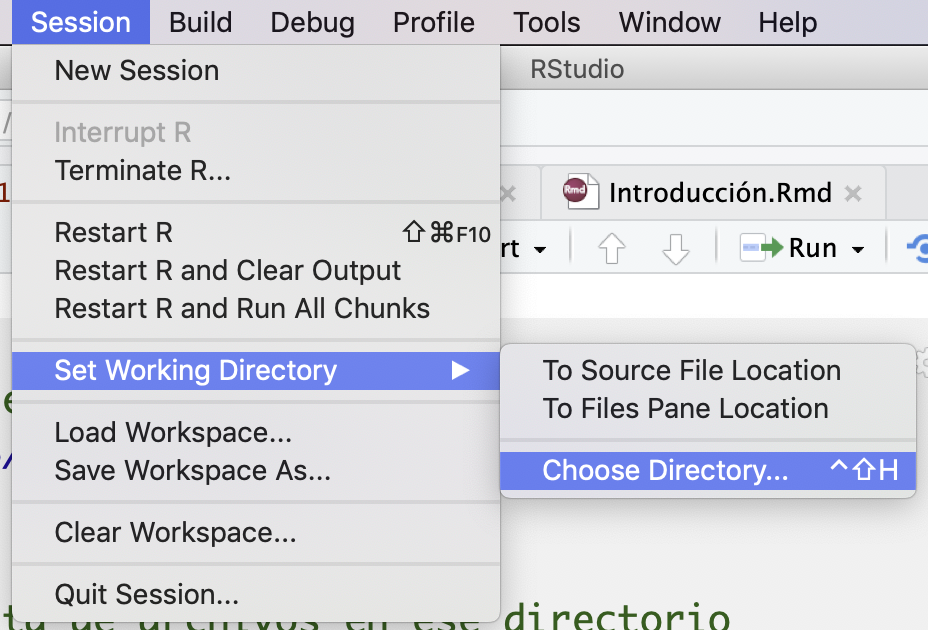
\includegraphics{intro1.png}

}

\caption{i0}

\end{figure}

\hypertarget{proyectos}{%
\section{Proyectos}\label{proyectos}}

Pero\ldots{} a veces preferimos trabajar en proyectos, sobre todo porque
nos da más control.

Hay gente que lo dice mejor que yo, como Hadley Wickham:
\url{https://es.r4ds.hadley.nz/flujo-de-trabajo-proyectos.html}

\hypertarget{instalaciuxf3n-de-paquetes}{%
\section{Instalación de paquetes}\label{instalaciuxf3n-de-paquetes}}

Los paquetes son útiles para realizar funciones especiales. La
especialización de paquetes es más rápida en R que en otros programas
por ser software libre.

Vamos a instalar el paquete \texttt{\{foreign\}}, como su nombre lo
indica, nos permite leer elementos ``extranjeros'' en R.

Para instalar las paqueterías usamos el siguiente comando
\texttt{install.packages()} Checa que adentro del paréntesis va el
nombre de la librería, con comillas.

Vamos a instalar dos librerías que nos permiten importar formatos.

\begin{Shaded}
\begin{Highlighting}[]
\CommentTok{\#install.packages("foreign", dependencies = TRUE)}
\CommentTok{\#install.packages("haven", dependencies = TRUE)}
\end{Highlighting}
\end{Shaded}

Este proceso no hay que hacerlo siempre. Si no sólo la primera vez. Una
vez instalado un paquete de librería, la llamamos con el comando
``library''

\begin{Shaded}
\begin{Highlighting}[]
\FunctionTok{library}\NormalTok{(haven)}
\FunctionTok{library}\NormalTok{(foreign)}
\end{Highlighting}
\end{Shaded}

\texttt{\{foreing\}} nos permite leer archivos en formato de
\emph{dBase}, con extensión ``.dbf''. Si bien no es un formato muy común
para los investigadores, sí para los que generan la información, puesto
que dBase es uno de los principales programas de administración de bases
de datos.

He puesto un ejemplo de una base de datos mexicana en dbf, en este
formato.

\begin{Shaded}
\begin{Highlighting}[]
\NormalTok{ejemplo\_dbf}\OtherTok{\textless{}{-}}\NormalTok{foreign}\SpecialCharTok{::}\FunctionTok{read.dbf}\NormalTok{(}\StringTok{"datos/ejemplo\_dbf.DBF"}\NormalTok{) }\CommentTok{\#checa cómo nos vamos adentro de nuestro directorio}
\end{Highlighting}
\end{Shaded}

Los \texttt{::} sirven para tres cosas:

\begin{itemize}
\item
  cargar un comando de un paquete, sin haberlo cargado
\item
  para identificar de qué paquete viene el comando.
\item
  para especificar en caso que hayan dos comandos iguales en un paquete,
  usar el que tenemos de los paquetes.
\end{itemize}

\hypertarget{paquete-pacman}{%
\section{\texorpdfstring{Paquete
\texttt{\{pacman\}}}{Paquete \{pacman\}}}\label{paquete-pacman}}

En general, cuando hacemos nuestro código querremos verificar que
nuestras librerías estén instaladas. Si actualizamos nuestro R y Rstudio
es probable (sobre todo en MAC) que hayamos perdido alguno.

Este es un ejemplo de un código. Y vamos a introducir un paquete muy
útil llamado \texttt{\{pacman\}}

\begin{Shaded}
\begin{Highlighting}[]
\ControlFlowTok{if}\NormalTok{ (}\SpecialCharTok{!}\FunctionTok{require}\NormalTok{(}\StringTok{"pacman"}\NormalTok{)) }\FunctionTok{install.packages}\NormalTok{(}\StringTok{"pacman"}\NormalTok{) }\CommentTok{\# instala pacman si se requiere}
\end{Highlighting}
\end{Shaded}

\begin{verbatim}
Loading required package: pacman
\end{verbatim}

\begin{Shaded}
\begin{Highlighting}[]
\NormalTok{pacman}\SpecialCharTok{::}\FunctionTok{p\_load}\NormalTok{(tidyverse, readxl, writexl, haven, sjlabelled, foreign) }\CommentTok{\#carga los paquetes necesarios para esta práctica}
\end{Highlighting}
\end{Shaded}

Hay muchos formatos de almacenamiento de bases de datos. Vamos a
aprender a importar información desde ellos.

\hypertarget{estilos}{%
\section{Estilos}\label{estilos}}

Escribir código tiene su gramática. Por lo general en este curso
seguiremos el estilo de Google

\url{https://google.github.io/styleguide/Rguide.html}

\hypertarget{ejercicio-1}{%
\section{Ejercicio 1}\label{ejercicio-1}}

Reealice en nuevo script lo siguiente:

\begin{enumerate}
\def\labelenumi{\arabic{enumi}.}
\item
  Escriba un vector ``x'', con los elementos 2,3,7,9. Muestre el
  resultado
\item
  Escriba un vector ``y'', con los elementos 9, 7, 3, 2. Muestre el
  resultado
\item
  Escriba un vector ``year'' con los años que van desde 1990 a 1993.
  Muestre el resultado
\item
  Escriba un vector ``name'' con los nombres de 4 de sus compañeros de
  curso. Muestre el resultado
\item
  Cree una matrix ``m'' 2x4 que incluya los valores 101 a 108, que se
  ordene según fila
\item
  ¿Cuáles son las dimensiones de la matriz ``m''?
\item
  Cree una matriz ``m2'' juntado los vectores ``x'' y ``y'', por sus
  filas ¿Cuáles son las dimensiones de la matriz ``m2''?
\item
  Convierta esa matriz en un \emph{data.frame}
\item
  Escriba una lista
\end{enumerate}



\end{document}
